\documentclass[twoside]{uva-inf-bachelor-thesis}
%\usepackage[dutch]{babel}
\usepackage{tikz}
\usepackage{tikz-qtree}
\usepackage[backend=bibtex]{biblatex}
%\bibliographystyle{IEEEtran}

\begin{filecontents}{\jobname.bib}

@MastersThesis{Schaik,
  type = {Bachelor Thesis},
  author = {S.J.R. van Schaik},
  title = {{Distributed simulation of digital circuits}},
  school = {University of Amsterdam},
  year = {2015}
}

\end{filecontents}

\bibliography{\jobname}

% Title Page
\title{Multi-touch screen hierarchical virtual "PIDAC" simulation}
\author{Sandro Dobric}
\supervisors{Toto van Inge (UvA), Edwin Steffens (UvA)}
\signedby{}

\begin{document}
\maketitle

\begin{abstract}
\begin{center}
\end{center}
\end{abstract}

\tableofcontents

\chapter{Introduction}
PIDAC (Plug-In Digital Analog Computer) is a learning tool for sequential and combinational logic. It is a system that has been in use for the past 30 years.
\\
\\
A succinct summary of the PIDAC system is given by the following excerpt from bachelor thesis "Distributed simulation of digital circuits" by van Schaik  \cite{Schaik}:
\\
\begin{quote}
PIDAC consists of a base board acting as a power grid for a collection of modules that can be plugged onto it, where a module is electronic circuit, most often an IC (integrated circuit), wrapped up in a user-friendly box, exposing its pins as jacks that allow them to be easily wired together with pluggable cables. Both digital and analog modules exist allowing people to quite simply learn about analog and digital electronics without having to solder and without having to know about the more in-depth details of electronics. Among these digital modules, one can find modules such as ALUs (arithmetic logic units), microcontrollers, registers, and NAND-gates. \end{quote}
\section{Research Questions}
To achieve the desired outcome for this project, the following research questions must be answered:
\begin{itemize}
  \item \textbf{Research question 1:} What kind of simulation is best suited to encompass all the features and characteristicsg of PIDAC?
  \item \textbf{Research question 2:} To what extent is automatic circuit verification possible?
  \item \textbf{Research question 3:} How does the designed simulation perform?
\end{itemize}


\chapter{Background and Related Work}

\chapter{Design Considerations}
\section{Platform and Development Language}
\section{Simulation Type}
There is a vast amount of simulation types that can be used to model a system. Some of these simulation types have the required attributes for modeling digital circuits. The exact attributes that we are looking for in a simulation type are shaped by the requirements of our digital circuit simulation.
\\
\\
The following list displays all the visual requirements for our simulation:

\begin{itemize}
  \item Symbolic visualisation of component logic
  \item Rubber band connections between components
  \item Hierarchical component wrapping
  \item Synchronous (clocked) and asychronous circuits
  \item A number of basic components
  \item Being able to create components from boolean logic
  \item Being able to store and load wrapped components and circuits
  \item Displaying of timing diagram for probe location
  \item Error messages/hints
  \item Ability to add delay
  \item Support for tri state connections
\end{itemize}
$~$
\\
In the domain of digital circuit simulation, there are two commonly used simulation types. These two types are discrete event simulation and cycle based simulation.

A discrete event simulation is one where the state variables only change at evenly spaced (discrete) intervals. The state variables are modified as a result of events taking place, these events take place in zero time. Events can lead to other events being created. Each event has a timestamp and will only be handled by the simulation at a certain time step. The implications for simulating digital circuits with this method are as follows:
\begin{itemize}
  \item Only state changes in the circuit are processed.
  \item Timing information is available.
\end{itemize}

A cycle based simulation takes advantage of the fact that most circuits are synchronous in design. 

The main advantage of a cycle based simulation over a discrete event simulation is execution speed. The drawback is that timing information is lost so static timing analysis is required if timing information is to be extracted.
\\
\\
\\
\\

As far as discrete-event simulation is concerned there are a number of world views.  A world view is the modeling framework that is used to represent a system and it's behaviour.
%Distributed discrete event simulation has been looked into, however considering the small scale of the circuits that are to be simulated, it was decided not to implement a distributed DES.

\chapter{Implementation}
\section{System Overview}
The system is comprised of the following components: Touch interface, discrete event simulation and circuit verification.


\section{Discrete Event Simulation}
As discussed in the design considerations section, the type of simulation that has been implemented is an object oriented discrete event simulation. The object oriented portion of the simulation indicates that the system state is modeled by object oriented entities.

To implement a discrete event simulation we must identify all the events that may occur in the system that is being modeled. In a PIDAC setup there are only a few things that can change the system state. The user can add components, connect components or change the state of input devices. Clock components can generate pulses and signals can propagate through components.
\\
This leaves us with the following events:
\begin{itemize}
  \item Clock pulse event
  \item User input event
  \item Component creation/deletion event
  \item Component connection/disconnection event
  \item Signal propagation event
\end{itemize}
$~$
\\
To define the state of our simulation, all the involved object entities must be defined. We can identify the following components:
\begin{itemize}
  \item Input/output component
  \item Logical component
  \item Hierarchical component
  \item Wire
  \item Input/output connector
\end{itemize}
$~$
\\
Seeing as all the components have either input or output connectors or even both, we can create an abstract object class 'component' that has connector attributes. Then we can make an abstract class 'single component' which inherits from 'component' and has the added property of having an evaluation function that determines how the output is derived from it's input. 
'Hierarchical component' also inherits from 'component' and has the added property of having a list of 'component' objects which form a component hierarchy. 'Input/output components' and 'logical components' both inherit from 'single component', the main difference being that 'logical component' has a boolean evaluation function and 'input/output component' has a hardcoded special evaluation function. The inheritance relationship for components is also depicted in fig. \ref{fig:compclass}.

\begin{figure}[h]
  \begin{center}
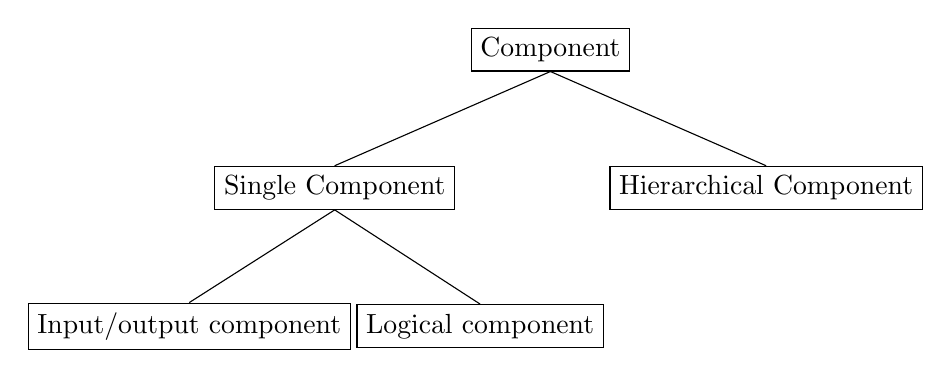
\begin{tikzpicture}
\tikzset{level distance=50pt}
\Tree [.\node[draw]{Component};
    [.\node[draw]{Single Component}; \node[draw]{Input/output component}; \node[draw]{Logical component};]
    [.\node[draw]{Hierarchical Component}; ]
    ]
]
\end{tikzpicture}
  \caption{Relationship between component classes \label{fig:compclass}}
  \end{center}
\end{figure}
$~$
\\
The simulation state consists of a list of components. Connections between components are modeled by 'wire' components. There can be multiple independant circuits in one simulation. This makes the state somewhat similar to a set of graphs, where the components are the nodes and the wires are the edges. As previously stated, each component has input/output connectors, this is where the bitvalues are stored.

Events are organized in a priority queue, where the event with the lowest associated timestep t is at the front of the queue. Each event has a different impact on the state. Clock pulse events create a signal propagation event for the current timestep for a selected clock component. User input events change the state of an input component. Component creation/deletion events create or delete the specified component.  Component connection/disconnection events create or destroy a 'wire' object between two components. Signal propagation events propagate 

%\section{Types of simulation}
%As far as simulation is concerned there are a number of world views
%\section{Modeling Digital Circuits}

\chapter{Circuit verification}

\chapter{Front End}
\section{Touch Interface}

\chapter{Evaluation}
\section{Functional Validation Test}
\section{Simulator Performance}

\chapter{Conclusions}

%\bibliographystyle{unsrt}
%\bibliography{\jobname}
\printbibliography

\end{document}
